\documentclass[border=6pt]{standalone}
\usepackage{amsmath}
\usepackage{tikz}
\usetikzlibrary{arrows.meta}
\begin{document}
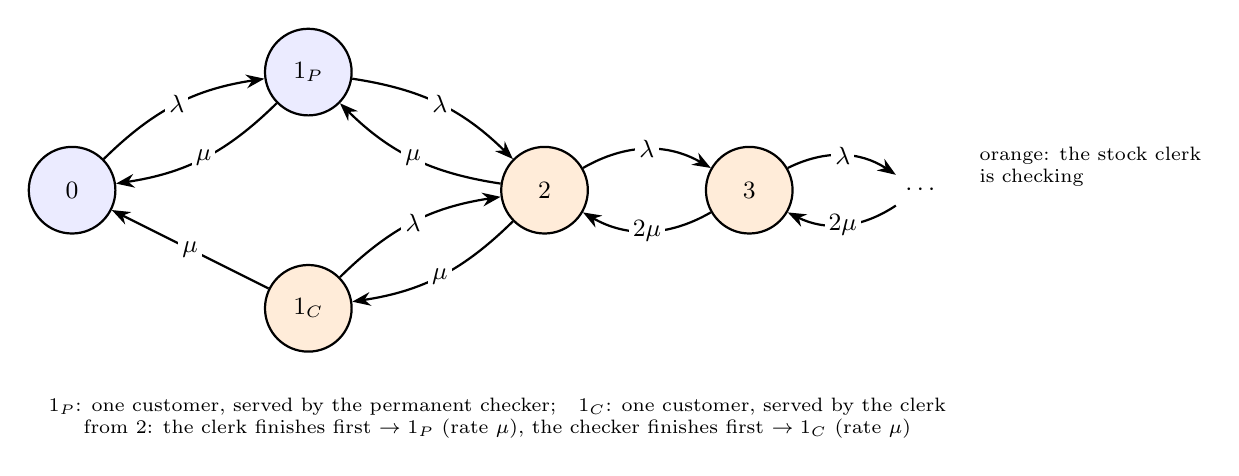
\begin{tikzpicture}[>=Stealth,font=\small,
 s/.style={draw,thick,circle,minimum size=1.1cm,inner sep=0pt,fill=blue!8},
 e/.style={->,thick},
 lab/.style={font=\small,fill=white,inner sep=1.5pt},
 every loop/.style={->,thick,looseness=6}]
\node[s] (0) at (0,0) {$0$};
\node[s] (1P) at (3.0,1.5) {$1_P$};
\node[s,fill=orange!15] (1C) at (3.0,-1.5) {$1_C$};
\node[s,fill=orange!15] (2) at (6.0,0) {$2$};
\node[s,fill=orange!15] (3) at (8.6,0) {$3$};
\node (d) at (10.8,0) {$\cdots$};
\draw[e] (0) to[bend left=18] node[lab]{$\lambda$} (1P);
\draw[e] (1P) to[bend left=18] node[lab]{$\mu$} (0);
\draw[e] (1C) -- node[lab]{$\mu$} (0);
\draw[e] (1P) to[bend left=18] node[lab]{$\lambda$} (2);
\draw[e] (2) to[bend left=18] node[lab,align=center]{$\mu$} (1P);
\draw[e] (1C) to[bend left=18] node[lab]{$\lambda$} (2);
\draw[e] (2) to[bend left=18] node[lab]{$\mu$} (1C);
\foreach \a/\b in {2/3,3/d} {
  \draw[e] (\a) to[bend left=30] node[lab]{$\lambda$} (\b);
  \draw[e] (\b) to[bend left=30] node[lab]{$2\mu$} (\a);
}
\node[font=\scriptsize,align=left,anchor=west] at (11.4,0.3) {orange: the stock clerk\\is checking};
\node[font=\scriptsize,align=center] at (5.4,-2.9) {$1_P$: one customer, served by the permanent checker;\quad $1_C$: one customer, served by the clerk\\from 2: the clerk finishes first $\to1_P$ (rate $\mu$), the checker finishes first $\to1_C$ (rate $\mu$)};
\end{tikzpicture}
\end{document}
